\documentclass[12pt]{article}

\usepackage[margin=0.8in]{geometry}
\usepackage[utf8]{inputenc}
\usepackage{hyperref}
\usepackage{graphicx}
\usepackage{amsmath}
\usepackage{pgfplots}
\usepackage{xcolor}
\usepackage{listings}
\usepackage{amssymb}
\usepackage{float}

\lstset{language=[90]Fortran,
  basicstyle=\ttfamily,
  keywordstyle=\color[HTML]{B22222},
  commentstyle=\color[HTML]{555555},
  morecomment=[l]{!\ }% Comment only with space after !
}

\pgfplotsset{width=10cm,compat=1.9}
\graphicspath{{./img}}

\usepgfplotslibrary{external}
\usetikzlibrary{calc}

\title{Perceptron}
\author{Erick Alejandro Carrillo López}
\date{2023/04/03}

\begin{document}
\maketitle
\tableofcontents
\newpage

\section{How works?:}
\subsection{A real neuron:}
A real neuron, also known as a nerve cell, is a specialized cell that transmits
electrical and chemical signals in the nervous system.\\
At the most basic level, a neuron consists of a cell body, dendrites, and an axon.
The cell body contains the nucleus and other organelles, and serves as the metabolic center
of the neuron. Dendrites are thin, branching extensions that receive signals from other
neurons or sensory cells. The axon is a long, thin projection that carries signals away
from the cell body to other neurons or target cells.
\begin{figure}[h]
  \centering
  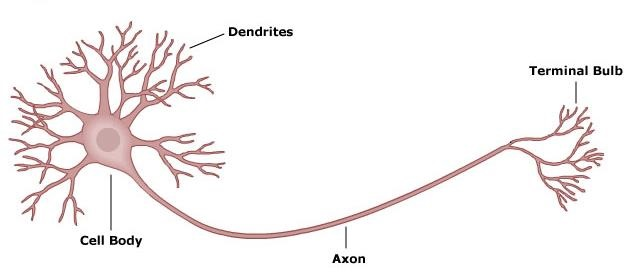
\includegraphics[scale = 0.5]{cell-body.jpg}
  \caption{Cell Body with its axon}
\end{figure}
Neurons communicate with each other through synapses, which are specialized
junctions between neurons. When an electrical signal, known as an action potential,
reaches the end of an axon, it triggers the release of neurotransmitter molecules, which diffuse
across the synapse and bind to receptors on the dendrites or cell body of the target neuron. This
binding can cause the target neuron to generate its own action potential, which propagates down its
axon to signal other neurons or target cells.
\begin{figure}[h]
  \centering
  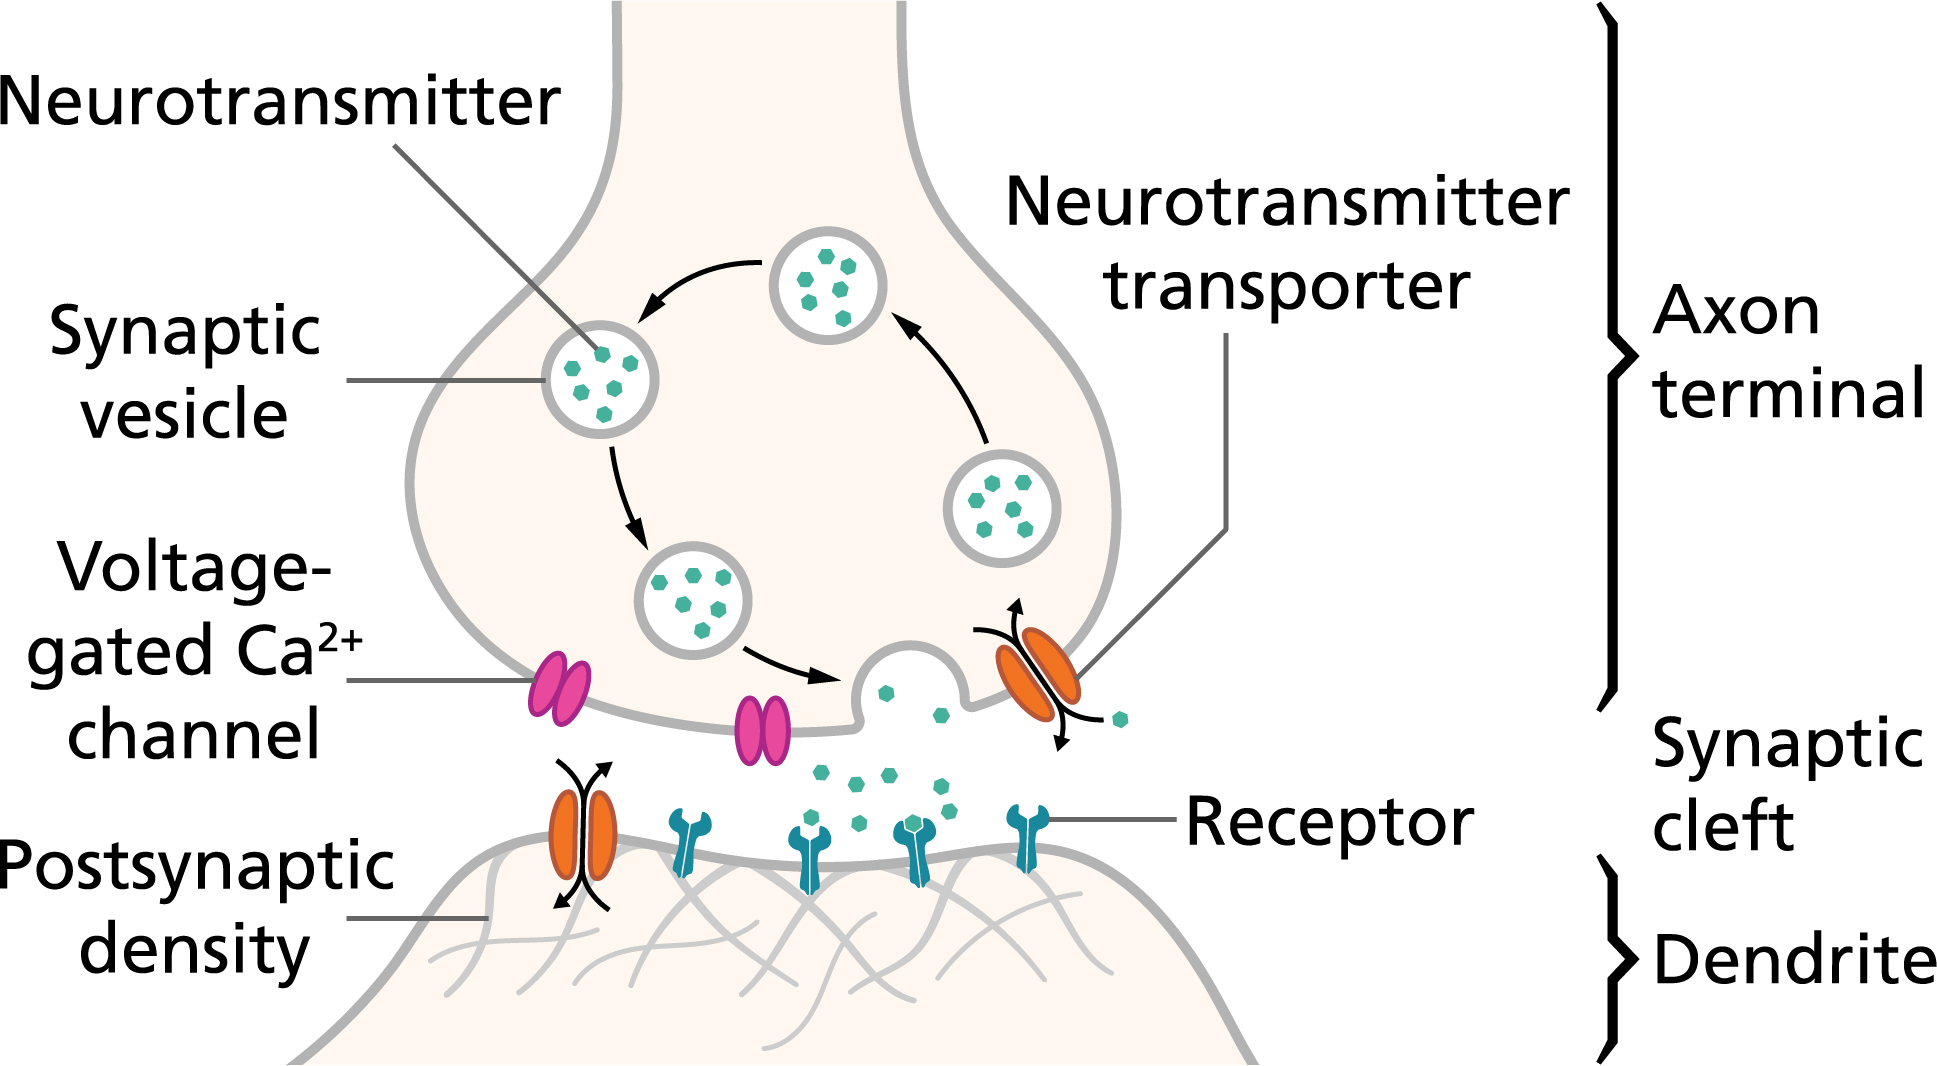
\includegraphics[scale = 0.19]{Synapse.jpg}
  \caption{Synapse}
\end{figure}

Neurons talk to each other across synapses. When an action potential reaches the
presynaptic terminal, it causes neurotransmitter to be released from the neuron into the synaptic
cleft, a 20–40nm gap between the presynaptic axon terminal and the postsynaptic dendrite
(often a spine).\\
After travelling across the synaptic cleft, the transmitter will attach to neurotransmitter
receptors on the postsynaptic side, and depending on the neurotransmitter released
(which is dependent on the type of neuron releasing it), particular positive (e.g. Na+, K+, Ca+)
or negative ions (e.g. Cl-) will travel through channels that span the membrane.
\subsection{The perceptron:}
The perceptron is a type of artificial neural network that is loosely modeled after the structure
and function of real neurons in the brain. The basic idea behind the perceptron is to use a
mathematical algorithm to simulate the behavior of a simplified neuron, which can then be used to
perform simple classification tasks.\\
The perceptron consists of an input layer, a set of weights, a summing or activation function,
and an output.
The input layer consists of one or more nodes, each of which represents a feature of the input data.
The weights are values that are assigned to each input node, which control the strength of the
connection between that node and the output.
\begin{figure}[h]
  \centering
  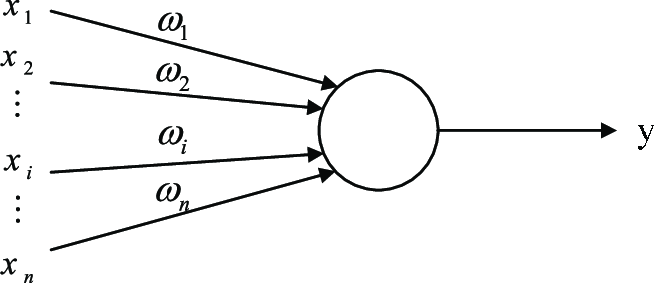
\includegraphics[scale = 0.5]{perceptron.png}
  \caption{Perceptron}
\end{figure}

The summing or activation function takes the weighted inputs and adds them together to produce a
single output
value. This output value is then compared to a threshold value, which determines whether the
perceptron will output a positive or negative value. If the output is positive, the perceptron
classifies the input as belonging to one class; if it is negative, the input is classified as
belonging to the other class.
\subsection{Perceptron parts:}
\begin{itemize}
\item \textbf{Input Nodes or Input Layer:} \\
  This is the primary component of Perceptron which accepts the initial data into the system for
  further processing. Each input node contains a real numerical value.
\item \textbf{Wight and Bias:} \\
  Weight parameter represents the strength of the connection between units. This is another most
  important parameter of Perceptron components. Weight is directly proportional to the strength of the
  associated input neuron in deciding the output. Further, Bias can be considered as the line of
  intercept in a linear equation.
\item \textbf{Activation Function:} \\
  These are the final and important components that help to determine whether the neuron will
  fire or not. Activation Function can be considered primarily as a step function.\\
  \textbf{Types of Activation functions:}
  \begin{itemize}
  \item Sign function.
  \item Step function.
  \item Sigmoid function.
  \end{itemize}
  \begin{figure}[h]
    \centering
    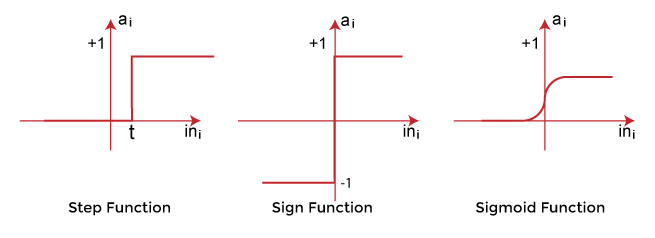
\includegraphics[scale = 0.5]{funcs.png}
    \caption{Types of activation functions}
  \end{figure}
\end{itemize}
\section{Códing the perceptron:}
\subsection{The Perceptron Algorithm:}
Perceptron model works in two important steps as follows.
\begin{enumerate}
\item In the first step first, multiply all input values with corresponding weight values and then add
  them to determine the weighted sum. Mathematically, we can calculate the weighted sum as follows.\\
  \[
    \sum_{i = 0}^{n}(weight_i \cdot input_i) = \sum_{i = 0}^{n}(w_i \cdot x_i) = w_0 \cdot x_0 + w_1 \cdot x_1
    + \cdots + w_n \cdot x_n
  \]\\
  Add a special term called bias 'b' to this weighted sum to improve the model's performance.\\
  \[
    \sum_{i = 0}^{n}(w_i \cdot x_i) + b
  \]
\item In the second step, an activation function is applied with the above-mentioned weighted sum,
  which gives us output either in binary form or a continuous value as follows.\\
  \[
    y = activation(\sum_{i = 0}^{n}(w_i \cdot x_i) + b) = activation(\vec{w} \cdot \vec{x} + b)
  \]
\end{enumerate}
At the end what we are doing here is a simple dot product of two vectors.
\[
  \sum_{i = 0}^{n}(w_i \cdot x_i) + b = \vec{w} \cdot \vec{x}
\]
Where.
\[
  \vec{w} = (b, w_1, \cdots, w_n)
\]
\[
  w_0 = b
\]
\[
  \vec{x} = (1, x_1, \cdots, x_n)
\]
\[
  x_0 = 1
\]
At the end we can think that this is hiperplane.

\begin{figure}[!hb]
  \centering
  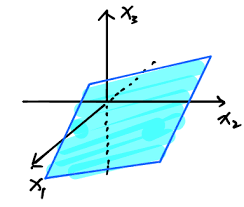
\includegraphics[scale = 1]{plane.png}
  \caption{A hyperplane}
\end{figure}

\subsection{From the perceptron algorithm to code:}
Firstly declare the threshold variable or bias variable,
this variable will be used as a threshold or bias for the activation function.
\begin{verbatim}
const threshold = 1.5
\end{verbatim}
After that declare two arrays the weights and inputs, the weights array is always initialized with random
values.
\begin{verbatim}
inputs = [1, 0, 1, 0, 1]
weights = [0.7, 0.6, 0.5, 0.3, 0.4]
\end{verbatim}
The weighted sum of the input values and weights by initializing a variable called sum to zero,
and then iterating over the input values and weights and adding the product of each input value
and weight to sum.
\begin{verbatim}
sum = 0.0
for (i = 0, i < inputs.length, i++)
    sum += inputs[i] * weights[i]
\end{verbatim}
And at the end just apply an activation function, a sign function to the weighted sum by checking
if sum is greater
than the threshold value of 1.5. If sum is greater than 1.5,
the activate variable is set to 1, otherwise, it is set to -1.
\begin{verbatim}
activate = (sum > threshold) ? 1 : -1
\end{verbatim}
Overall, this code represents a simple example of how a perceptron might work by calculating a
weighted sum of inputs and weights and applying a threshold activation function to produce a
binary output.
\subsection{How to train a perceptron? and The perceptron learning algorithm:}
To train a perceptron, we need to adjust the weights of the input connections so that the
perceptron produces the desired output for a given set of inputs. We can do this by using an
iterative algorithm called the perceptron learning algorithm.\\
The key idea behind the perceptron learning algorithm is that we can use the error between the
predicted and desired outputs to adjust the weights so that the perceptron becomes better at
producing the desired output. Specifically, we adjust the weights in proportion to the error, with
larger errors resulting in larger weight updates.\\
Note that the perceptron learning algorithm assumes that the problem is linearly separable, which
means that there is a hyperplane that can separate the positive and negative examples in the input
space. If the problem is not linearly separable, the perceptron may not be able to converge to a
solution.\\
\begin{figure}[h]
  \centering
  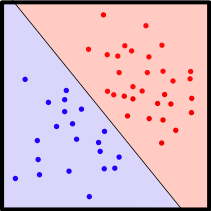
\includegraphics{linearly.png}
  \caption{Linear separability}
\end{figure}
\subsubsection{The Mathematical definition behind linear separability:}
Let $X_0$ and $X_1$ be two sets of points in an n-dimensional Euclidean space. Then $X_0$ and $X_1$
are linearly separable, if there exist $n + 1$ real numbers $w_1, w_2, \cdots, w_n, k$ such that
every point $x \in X_0$ satisfies $\sum_{i = 1}^{n}(w_i \cdot x_i) > k$ and every point $x \in X_1$
satisfies
$\sum_{i = 0}^{n}(w_i \cdot x_i) < k$ where $x_i$ is the i-th component of $x$.
\subsection{From the learning algorithm to code:}
You must create a training function with these characteristics using the previous data.
\begin{enumerate}
\item The training function guesses the outcome based on the activate function.
\item Every time the guess is wrong, the perceptron should adjust the weights.
\item After many guesses and adjustments, the weights will be correct.
\end{enumerate}
Define the activation function which at the end it is a simple binary function.
\begin{verbatim}
int activation(x)
    return (x > 0) ? 1 : -1
\end{verbatim}
Define the learning rate and a number of epochs, which is the amount of times that we are going
train the perceptron and the learning rate represents how fast our perceptron is going to learn.
\begin{verbatim}
learning_rate = 0.1
num_epochs = 100
\end{verbatim}
Train the perceptron by iterating with all the training data which in this case it is an bidimensinal
array and a simple threshold or bias.
\begin{verbatim}
for (i = 0, i < num_epochs, i++)
    for (j = 0, j < inputs.length, j++)
        sum = 0.0
        for (k = 0, k < weights.length, k++)
            sum += inputs[j][k] * weights[i]
        sum += b
        out = activation(sum)
\end{verbatim}
And at the end we only need to adjust the weights and bias from the error, so the error is so simple
it is  a subtraction, then use the error and the learning rate to update the weights and bias.
\begin{verbatim}
error = label[j] - output
for (k = 0, k < weights.length, k++)
    weights[k] += learning_rate * error * inputs[j][k]
b += learning_rate * error
\end{verbatim}
\subsection{The math behind the learning algorithm:}
Maybe now the main question is why we adjust the weights like that.
\begin{verbatim}
weights[k] += learning_rate * error * inputs[j][k]
\end{verbatim}
And the bias or threshold.
\begin{verbatim}
b += learning_rate * error
\end{verbatim}
To answer that we need to formulate a math function that represents our neuron which receives a vector
as input.
\[
  f(\vec{x}) = 
  \begin{cases}
    1 &\quad if \vec{w} \cdot \vec{x} > 0  \\
    -1 &\quad \text{otherwise} \\
  \end{cases}
\]

Where $\vec{w} = (b, w_1, \cdots, w_n)$
is the coefficients or weights, $\vec{x} = (1, x_1, \cdots, x_n)$
the input vector, so from this idea we can come up
with something like this.
\[
  y_t = 1 \implies \vec{w} \cdot \vec{x}_t > 0
\]

\[
  y_t =  - 1 \implies \vec{w} \cdot \vec{x}_t \le 0
\]
Where $(\vec{x}_t, y_t) \in \mathbb{D}$ which is the whole dataset, then from these implications
we can formulate two inequalities that
represent when the perceptron is wrong and when it is correct.
\[
  \text{Correct} \implies y_t \cdot \vec{x}_t \cdot \vec{w} > 0
\]

\[
  \text{Wrong} \implies y_t \cdot \vec{x}_t \cdot \vec{w} \le 0
\]

At the end what we want is a desired vector $\vec{\theta}^*$ which fulfills a single characteristic.
\[
  \exists \vec{\theta}^* \in \mathbb{R}^{d} \quad|\quad y_t\vec{\theta}^*\vec{x}_t > 0,\quad
  \forall (\vec{x}_t, y_t) \in \mathbb{D}
\]
Where $\vec{\theta}^*$ is the desired vector configuration which classifies the inputs perfectly
and $\mathbb{D}$ is the data set,
then when the perceptron gets an error this both inequalities are true.
\[
  y_t\vec{w}_k \vec{x} \le 0 \Leftrightarrow  y_t \not = y'
\]
Where $y'$ is the result obtained,
then in the algorithm when that happens we update the $\vec{w}$ like this.
\[
  \vec{w}_{k + 1} = \vec{w}_{k} + y_t\vec{x}_t
\]
In the algorithm we try to make those changes less aggressive, so to understand
why we adjust the weights like that, think on this chart.
\begin{center}
\begin{tikzpicture}[scale=1.5]
  \draw[thick,->] (2,0) -- (0,1) node[anchor=south west]{$\vec{w}_k$};
  \draw[thick,->] (2,0) -- (5,0) node[anchor=south west]{$\vec{\theta}^*$};
\end{tikzpicture} \\
\end{center}
Again the $\vec{\theta}^*$ is the desired vector configuration which for any
$(\vec{x}_t, y_t) \in \mathbb{D}$ returns an $y' = y_t$ and the $\vec{w}_k$ is the current k-th iteration
of the weights, obviously we don't know where $\vec{\theta}^*$ is, but we can approximate $\vec{w}_k$
to $\vec{\theta}^*$ by a 
simple additions of vectors,
then We can put the vector $y_t \cdot \vec{x}_t$ in the chart.
\begin{center}
\begin{tikzpicture}[scale=1.5]
  \draw[thick,->] (2,0) -- (0,1) node[anchor=south west]{$\vec{w}_k$};
  \draw[thick,->] (2,0) -- (5,0) node[anchor=south west]{$\vec{\theta}^*$};
  \draw[thick,->] (2,0) -- (5,-1) node[anchor=south west]{$y_t\vec{x}_t$};
\end{tikzpicture} \\
\end{center}
Then if we compute
the dot product of these two vectors $y_t\vec{x}_t \cdot \vec{\theta}^*$ this inequalitie
becomes true.
\[
  y_t\vec{\theta}^*\vec{x}_t > 0
\]
Because again the $\vec{\theta}^*$ is the desired vector configuration, the meaning of the dot product
of two vectors is how much they are pointing in the same direction,
if the dot product of two vectors is positive, it means they are pointing in
roughly the same direction, if it is negative, they are pointing in roughly opposite
directions, and if it is zero, they are perpendicular (at a right angle) to each other,
then the dot product of two Euclidean vectors $\vec{v}$ and $\vec{u}$ is defined by.
\[
  \vec{v} \cdot \vec{u} = ||\vec{v}|| \cdot ||\vec{u}|| \cdot \cos{\theta}
\]
Where $\theta$ is the angle between $\vec{v}$ and $\vec{u}$, so
from that idea we can perfectly infer that $y_t\vec{x}_t \cdot \vec{w}_k \le 0$ by their angle.\\
\begin{center}
\begin{tikzpicture}[scale=1.5]
  \draw[thick,->] (2,0) -- (0,1) node[anchor=south west]{$\vec{w}_k$};
  \draw[thick,->] (2,0) -- (5,0) node[anchor=south west]{$\vec{\theta}^*$};
  \draw[thick,->] (2,0) -- (5,-1) node[anchor=south west]{$y_t\vec{x}_t$};

  \draw let \p1 = (-2,1), \p2 = (5,-1.78), \n1 = {atan2(\y1,\x1)}, \n2 = {atan2(\y2,\x2)} in (2,0) + (\n1:0.8) arc (\n1:\n2:0.8) node[midway, above right] {$\theta$};
\end{tikzpicture} \\
\end{center}
So think in the addition of vector as way to rotate a vector, look if I sum $\vec{w}_k + y_t\vec{x}_t$
I get the next iteration the $k + 1$ iteration which results on this new vector $\vec{w}_{k + 1}$.
\begin{center}
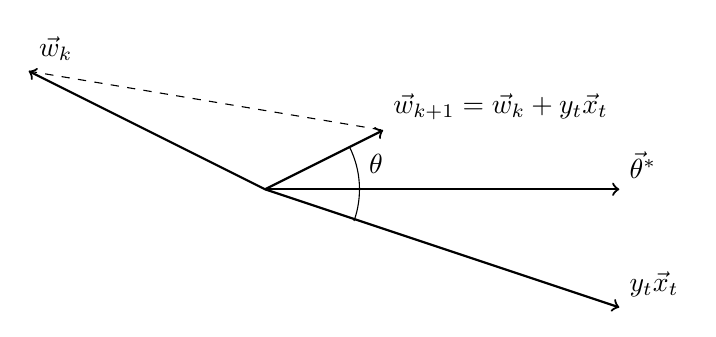
\begin{tikzpicture}[scale=1.5]
  \draw[thick,->] (2,0) -- (0,1) node[anchor=south west]{$\vec{w}_k$};
  \draw[thick,->] (2,0) -- (5,0) node[anchor=south west]{$\vec{\theta}^*$};
  \draw[thick,->] (2,0) -- (5,-1) node[anchor=south west]{$y_t\vec{x}_t$};
  \draw[thick,->] (2,0) -- (3,0.5) node[anchor=south west]{$\vec{w}_{k + 1} = \vec{w}_k + y_t\vec{x}_t$};
  \draw[dashed] (0,1) -- (3,0.5);
  
  \draw let \p1 = (2,1), \p2 = (5,-1.78), \n1 = {atan2(\y1,\x1)}, \n2 = {atan2(\y2,\x2)} in (2,0) + (\n1:0.8) arc (\n1:\n2:0.8) node[midway, above right] {$\theta$};
\end{tikzpicture} \\
\end{center}
With this new vector $\vec{w}_{k+1}$ we generate a new angle $\theta$ that makes
this inequalitie $\vec{w}_{k+1} \cdot y_t\vec{x}_t \le 0$
false 
which implies that the perceptron have learned the pattern, basically we adjust the weights
 to new direction.
\[
  \neg (\vec{w}_{k+1} \cdot y_t\vec{x}_t \le 0) \implies \vec{w}_{k+1} \cdot y_t\vec{x}_t > 0\quad |
  \quad y' = y_t, \quad \vec{w}_k \rightarrow \vec{\theta}^*
\]
We are arriving to a conjecture which is that it looks like we need a finite amount of $k$
iterations to perfectly separate the points or vectors $\vec{x}_t$ in $\mathbb{D}$
making $\vec{w}_k \rightarrow \vec{\theta}^*$, creating that perfectly
hyperplane that separates the points.
This is so important because if that amount of iterations is infinite then the
algorithm is useless because means that we are not going to have any chance to classifie most of
the possible inputs,
but if it is a finite amount of iterations means that we are going to have the chance to
classifie most of the posible inputs
making this useful,  spoiler, there are finite amounts of iterations for a separable finite
set of tuples $(\vec{x}_t, y_t) \in \mathbb{D}$, so lets proof that.
\subsection{Perceptron Convergence Proof:}
Lets think in that variable $k$ which represents the amount of iterations,
It should be a finite natural number.
\[
  k \in \mathbb{N}
\]
Then before to continue with the proof we need to do an assumption,
we are going to scale our $\vec{\theta}^*$ in another words we are going to change it
for an easy manipulation,
so for this section we are going to work with a new vector.
\[
  \vec{\theta}^* = \alpha \cdot \vec{\theta}\quad |\quad ||\vec{\theta}|| = 1
\]
So we scale the desired vector $\vec{\theta}^*$ for getting its unitary vector $\vec{\theta}$,
At the end the inequality is still being true.
\[
  y_t\vec{\theta}^*\vec{x}_t > 0
\]
\[
  y_t\alpha\cdot\vec{\theta}\vec{x}_t > 0
\]
\[
  \frac{1}{\alpha} \cdot y_t\alpha\vec{\theta}\vec{x}_t > 0 \cdot \frac{1}{\alpha}
\]
\[
  y_t\vec{\theta}\vec{x}_t > 0
\]
Obviously all the computed values with this new vector $\vec{\theta}$ are going to be lesser than
the comptued values with $\vec{\theta}^*$, to be exact is going to be $\alpha$ times greater, and
actually if you think we don't care how big these outputs are, we only care
that they are big enoguh to make that statement true the whole time.
\[
  y_t\vec{\theta}^*\vec{x}_t > y_t\vec{\theta}\vec{x}_t > 0
\]

To just finished with this idea think on this statement
and lets continue with the proof of the convergence.
\[
  \exists \vec{\theta}^* = \alpha \cdot \vec{\theta}\quad|\quad
  y_t\vec{\theta}^*\vec{x}_t > 0 \wedge
  y_t\vec{\theta}\vec{x}_t > 0,
  \quad \forall(\vec{x}_t, y_t)
  \in \mathbb{D}
\]

Then we need to think in this
dot product $\vec{w}_{k + 1} \cdot \vec{\theta}$ because this dot product
will grow but it will never decrease and why is that?, well because of the algorithm we only
rotate or adjust $\vec{w}_{k}$ when $\vec{w}_k \cdot \vec{x}_ty_t \le 0$, look this chart.
\begin{center}
\begin{tikzpicture}[scale = 0.8]
  \draw[->, thick] (-5,0)--(5,0) node[right]{$t$};
  \draw[->, thick] (0,-5)--(0,5) node[above]{$\vec{w}_{k + 1} \cdot \vec{\theta}$};
  
  \draw[black, thick] (0, -2) -- (0, -1) -- (0.5,-0.5) -- (1,0) -- (1.5, 1.5) -- (2, 2) -- (2.5, 3) -- (3, 3.5) -- (4, 3.5) -- (5, 5);
\end{tikzpicture}
\end{center}
You can imagine something like this, it never decreases, so why this dot product is useful?, well
because this dot product represents how the weights are being adjust or how the perceptron learns,
it would start in some negative real number but it will finish in some positive value,
and as I said before there is going to be a moment where $\vec{w}_{k+1} \cdot \vec{\theta}$
will never increase
anymore, at the end we would find inserting how this dot product grows through
the instances of $(\vec{x}_t, y_t)$.
\begin{center}
\begin{tikzpicture}[scale = 0.8]
  \draw[->, thick] (-5,0)--(10,0) node[right]{$t$};
  \draw[->, thick] (0,-5)--(0,5) node[above]{$\vec{w}_{k + 1} \cdot \vec{\theta}$};
  
  \draw[black, thick] (0, -2) -- (0, -1) -- (0.5,-0.5) -- (1,0) -- (1.5, 1.5) -- (2, 2) -- (2.5, 3) -- (3, 3.5) -- (4, 3.5) -- (5, 5) -- (10, 5);
\end{tikzpicture}
\end{center}
Let's imagine that we already have made a some $k$ iteration,
then we want to know what would be 
the minimum difference between this $k$ iterations $\vec{w}_{k+1} \cdot \vec{\theta}$ with It's
previous iteration $\vec{w}_{k} \cdot \vec{\theta}$, well.
\[
  \vec{w}_{k + 1} \cdot \vec{\theta} = (\vec{w}_{k} + y_t\vec{x}_t) \vec{\theta}
  = \vec{w}_{k}\vec{\theta} + y_t\vec{x}_t\vec{\theta}
\]
\[
  \vec{w}_{k + 1} \cdot \vec{\theta} -  \vec{w}_{k}\vec{\theta}
  =  y_t\vec{x}_t\vec{\theta}
\]
So basically this is
the difference $y_t\vec{x}_t\vec{\theta}$ which is $y_t\vec{x}_t\vec{\theta} > 0$ and so
from this expression we can create constant gamma which represents the minimum
difference of some pair of values $\vec{w}_{k+t} \cdot \vec{\theta} - \vec{w}_{k} \cdot \vec{\theta}$
by any $k$ iteration.
\[
  \gamma = minimum(y_t \vec{x}_t\vec{\theta}) \quad|\quad \forall (\vec{x}_t, y_t) \in \mathbb{D}
\]
We know that $y_t \in \{1, -1\}$, so we can forget it and use a simple absolute value.
\[
  \gamma = minimum(|\vec{x}_t\vec{\theta}|) \quad|\quad \forall (\vec{x}_t, y_t) \in \mathbb{D}
\]
\[
  |\vec{w}_{k + 1} \cdot \vec{\theta} -  \vec{w}_{k}\vec{\theta}|
  \ge \gamma\quad | \quad \forall \vec{w}_{k+1}
\]

Finally we can abstract this idea of $\gamma$ to an inequalitie for all the $k$ iterations.
\[
  \gamma \cdot k \le |\vec{w}_{k+1} \cdot \vec{\theta}| \le ||\vec{w}_{k+1}||\cdot ||\vec{\theta}||
  = ||\vec{w}_{k+1}||\quad|\quad \forall \vec{w}_{k + 1}
\]
\[
  \gamma \cdot k \le ||\vec{w}_{k+1}||\quad|\quad \forall \vec{w}_{k + 1}
\]
As you can see we replace $||\vec{\theta}|| = 1$, because if unitary vector and
$\gamma \cdot k$ works as lower bound for any $|\vec{w}_{k + 1}\cdot \vec{\theta} |$, this lead us
to think if there exist a higher bound, spoiler, It exists, to find it now we need to think in another
dot product which is this.
\[
  \vec{w}_{k + 1} \cdot \vec{w}_{k+1}
\]
In some way this dot product is an scalar way to represent each state of our weights, It is chaotic
because this dot product would decrease and increase and something to take not It is that
always this dot product will be
$\vec{w}_{k + 1} \cdot \vec{w}_{k+1} > 0$, this is because is the same vector,
so you can think in a chart like this.
\begin{center}
\begin{tikzpicture}[scale = 1]
  \draw[->, thick] (0,0)--(10,0) node[right]{$t$};
  \draw[->, thick] (0,0)--(0,5) node[above]{$\vec{w}_{k + 1} \cdot \vec{w}_{k + 1}$};

  \draw[black, thick] (0,5) -- (1, 1) -- (2, 2.5) -- (3, 2.5) -- (4, 5) -- (6, 5) -- (8, 1) -- (9, 4);
\end{tikzpicture}
\end{center}
Now we are thinking
what is the larger difference between
any $k$ iteration $\vec{w}_{k+1} \cdot \vec{w}_{k+1}$ with It's
previous iteration $\vec{w}_{k} \cdot \vec{w}_{k}$, well.
\[
  \vec{w}_{k + 1} \cdot \vec{w}_{k + 1} = (\vec{w}_{k} + y_t\vec{x}_t) \cdot (\vec{w}_{k} + y_t\vec{x}_t)
  = \vec{w}_k\vec{w}_k + 2y_t\vec{w}_k\vec{x}_t + y_t^2\vec{x}_t\vec{x}_t
\]

\[
  \vec{w}_{k + 1} \cdot \vec{w}_{k + 1} - \vec{w}_k \cdot \vec{w}_k
  = 2y_t\vec{w}_k\vec{x}_t + y_t^2\vec{x}_t\vec{x}_t
\]
Then this is the difference $2y_t\vec{w}_k\vec{x}_t + y_t^2\vec{x}_t\vec{x}_t$,
so we can rewrite this expression
like this.
\[
  2y_t\vec{w}_k\vec{x}_t + \vec{x}_t\vec{x}_t
\]
Because $y_t \in \{1, -1\}$ so $y_t^2 = 1$ for all $(\vec{x}_t, y_t) \in \mathbb{D}$, so what is going
to be the maximum difference between any $\vec{w}_{k+1} \cdot \vec{w}_{k+1}$, so thinking in this
expression $2y_t\vec{w}_k\vec{x}_t + \vec{x}_t\vec{x}_t$ to be specific thinking on the first quotient,
this quotient always is going to be $2y_t\vec{w}_k\vec{x}_t \le 0$, so we eliminate this
expression and create an inequalitie, because we want the largest posible value.

\[
  \vec{w}_{k + 1} \cdot \vec{w}_{k + 1} - \vec{w}_k \cdot \vec{w}_k
  \le \vec{x}_t\vec{x}_t
\]
Then we can create our constant $R^2$
 which represents the largest
difference of some pair of values $\vec{w}_{k+t} \cdot \vec{w}_{k+1} - \vec{w}_{k} \cdot \vec{w}_k$
by any $k$ iteration and why $R^2$ ?, well.
\[
  R = maximum(||\vec{x}_t||) \quad|\quad \forall (\vec{x}_t, y_t) \in \mathbb{D}
\]
\[
  R = ||\vec{x}_t|| = \sqrt{\sum_{i = 0}^{n}x_i^2}
\]
\[
  R^2 = ||\vec{x}_t||^2 = \sqrt{\sum_{i = 0}^{n}x_i^2}^2 = \sum_{i = 0}^{n}x_i^2 = \vec{x}_t \cdot \vec{x}_t
\]
Finally, we chose this constant $R^2$, and we don't choose $maximum(|\vec{x}_t\vec{\theta}|)$,
because we are searching to a higher boundary, and as $\|\vec{\theta}|| \le ||\vec{x_t}||$ always
is going to be lesser to $R^2$, so finally we can mix everything together, so we can assume this.
\[
  \gamma^2k^2 \le ||\vec{w}_{k+1}||^2 = \vec{w}_{k+1} \cdot \vec{w}_{k+1}
\]
So we can take that and create our finall inequalitie, which at the end is this.
\[
  \gamma^2k^2 \le \vec{w}_{k+1} \cdot \vec{w}_{k+1} \le k \cdot R^2\quad |\quad \forall\vec{w}_{k+1}
\]
Here we are boundary the amount of change, if you want to see this like
that, of the weights of the perceptron
for all the instances of $\vec{w}_{k + 1}$, from this two bounds we can get a finite number
of steps or times that the perceptron needs for update its weights to converge, just like this.
\[
  \gamma^2k^2 \le k \cdot R^2
\]
\[
  \frac{1}{\gamma^2 \cdot k} \cdot \gamma^2k^2 \le k \cdot R^2 \cdot \frac{1}{\gamma^2 \cdot k}
\]
\[
  k \le \frac{R^2}{\gamma^2}
\]
That's it, $k$ is a real number which means that takes at least $\frac{R^2}{\gamma^2}$
updates or steps to converge.

\section{Examples:}
Now you know why the algorithm works like that, and we solved the conjecture of the finite amount
of iterations, so lets see how we can use the perceptron as a binary classifier,
you can find the
\href{https://github.com/alecksandr26/machine-learning-code/tree/main/examples}{examples here}.
\subsection{Perceptron module in fortran:}
Firstly I made a simple perceptron module in fortran which contains the weights, a bias and with a
simple sign activation function, it has some subroutines implemented for training and testing the
perceptron and here is the
\href{https://github.com/alecksandr26/machine-learning-code/blob/main/src/mod_perceptron.f90}{source
  code}

\begin{lstlisting}
#include <assertf.h>

module mod_perceptron
    use iso_fortran_env, only : real32, int32
 
    use assertf
    implicit none

    private
    public p_init, p_free, p_train, p_test, perceptron, p_get_weights

    ! The type where we are going to contain the weights and bieas
    type perceptron
        real(real32) ::  b
        integer(int32) :: n     ! The amount of weights
        real(real32), pointer :: w(:) ! The weights
    end type perceptron
contains
    
    ! step: A simple activation function
    pure function step(output)
        real(real32), intent(in) :: output
        real(real32) :: step
        if (output > 0.0) then
            step = 1.0
        else
            step = - 1.0
        end if
    end function step
    
    ! p_init: Receives a perceptron type and adds to it the weights and bias
    subroutine p_init(per, w, b)
        real(real32), intent(in) :: w(:), b
        type(perceptron), intent(out) :: per

        per%n = size(w)         ! Fetch the size of the array of weights
        
        ! Allocate the array of weights and copy it
        allocate(per%w(per%n))
        per%w(:) = w(:)
        per%b = b
    end subroutine p_init

    ! p_free: To free the perceptrons weights and set the size and bias to zero
    subroutine p_free(per)
        type(perceptron), intent(in out) :: per
        
        deallocate(per%w)
        per%n = 0
        per%b = 0
    end subroutine p_free
        
    ! p_train: To train the perceptron with some data
    subroutine p_train(per, inputs, outputs, lrate, nepochs)
        ! in out Because we are going to modify
        type(perceptron), intent(in out) :: per 
        ! The inputs and outputs to be trained
        real(real32), intent(in) :: inputs(:,:) ! Bindimensional array
        real(real32), intent(in) :: outputs(:), lrate ! Learning rate
        integer(int32), intent(in) :: nepochs        ! Num of epochs
        real(real32), allocatable :: results(:), errors(:), deltas(:)

        ! The size and more arrays to catch data for the training
        integer(int32) :: n, i, j, k
        ! Catch the amount of inputs, sizeof(inputs[1])
        n = size(inputs, 1)     

        allocate(results(n))
        allocate(errors(n))
        allocate(deltas(n))
        
        do concurrent(i = 1 : nepochs)            ! Start iterating
            do concurrent(j = 1 : n) ! Concurrent iteration
                ! Computing the perceptron calculation
                results(j) = per%b
                do concurrent(k = 1 : per%n)
                    results(j) = results(j) + per%w(k) * inputs(j, k)
                end do
                
                ! The activation function
                results(j) = sign_act(results(j))

                ! Compute the error 
                errors(j) = outputs(j) - results(j)
                deltas(j) = lrate * errors(j)

                ! Update the perceptron
                per%b = per%b + deltas(j)
                do concurrent(k = 1 : per%n)
                    per%w(k) = per%w(k) + deltas(j) * inputs(j, k)
                end do
            end do
        end do

        deallocate(results)
        deallocate(errors)
        deallocate(deltas)
    end subroutine p_train

    ! p_test: To test the perceptron with some inputs
    subroutine p_test(per, inputs, results)
        type(perceptron), intent(in) :: per
        real(real32), intent(in) :: inputs(:, :)
        real(real32), intent(out) :: results(:)

        ! The size and outputs
        integer(int32) :: n, i, j
        
        ! Test the perceptron
        n = size(inputs, 1)
        do concurrent(i = 1 : n)
            results(i) = per%b
            do concurrent(j = 1 : per%n)
                results(i) = results(i) + per%w(j) * inputs(i, j)
            end do
            results(i) = step(results(i))
        end do
    end subroutine p_test

    ! p_get_weights: To get the weights from the perceptron
    subroutine p_get_weights(per, weigths)
        type(perceptron), intent(in) :: per
        real(real32), intent(out) :: weigths(:)
        
        weigths(:) = per%w(:)
    end subroutine p_get_weights
end module mod_perceptron
\end{lstlisting}
\subsection{Logic gates:}
So lets see if the perceptron is capable to learn how the logic gates works, so the first
thing what I have done is to create the training inputs as a simple binary intputs like 1 and 0,
the intersting thing is in the outpus array where I put the outputs that a normal \textbf{and} logic gate
must give us.
\begin{lstlisting}
  program example
    use iso_fortran_env, only : real32, int32
    use mod_perceptron
    use assertf

    type(perceptron) :: per
    real(real32) :: inputs(4,2), outputs(4), results(4), weigths(2)

    weigths = [0.8, 0.3]
    call p_init(per, weigths, - 0.2)      ! Initialize the perceptron

    inputs = reshape([0.0, 1.0, 0.0, 1.0, 0.0, 0.0, 1.0, 1.0], [4,2])
    ! inputs = [[0.0, 1.0, 0.0, 1.0], [0.0, 0.0, 1.0, 1.0]]

    outputs = [- 1.0, - 1.0, - 1.0, 1.0] ! Outputs that should return

\end{lstlisting}
After initializing the perceptron I called the training function which receives a specific
amount of epochs which means the amount of times that the perceptron is going to retrain itself,
and a learning rate of 0.1 which is how aggressive adjust its weights.
\begin{lstlisting}
    ! Train the perceptron, with lrate = 0.1, nepochs = 1000
    call p_train(per, inputs, outputs, 0.1, 1000)

    ! Test the perceptron
    call p_test(per, inputs, results)
\end{lstlisting}
Finally I print everything and it looks like that he perfectly understand the logic gates.
\begin{lstlisting}
    ! Print all the data
    write(*,*) 'x1:', inputs(:, 1)
    write(*,*) 'x2:', inputs(:, 2)
    write(*,*) 'outputs:', outputs
    write(*,*) 'and_w1:', per%w(1)
    write(*,*) 'and_w2:', per%w(2)
    write(*,*) 'and_b:', per%b
    write(*,*) 'and_results:', results
\end{lstlisting}
\textbf{Output:}
\begin{verbatim}
x1:   0.00000000       1.00000000       0.00000000       1.00000000    
x2:   0.00000000       0.00000000       1.00000000       1.00000000    
outputs:  -1.00000000      -1.00000000      -1.00000000       1.00000000    
and_w1:  0.400000036    
and_w2:  0.300000012    
and_b: -0.600000024    
and_results:  -1.00000000      -1.00000000      -1.00000000       1.00000000
\end{verbatim}

\newpage
\subsubsection{Picture of the results with the logic gates:}
In the complete program I also tried the nand logic gate and the or logic gate, catch its outputs
data and plot it into some charts, these were the results, as you can see  it perfeclty finds the
hiperplane to separte the inputs.
\begin{figure}[H]
  \centering
  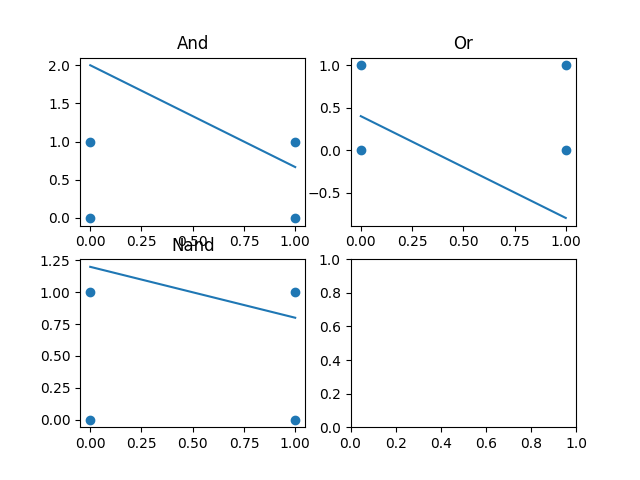
\includegraphics[scale = 1]{logic_gates.png}
  \caption{The results of the perceptron with logic gates}
\end{figure}

\newpage
\subsection{Classifying images:}
Now lets try to do something more realistic we want to classify images with circles and rectangles
each image has a rectangle o a circle, we want to train the perceptron to be able to classifie each
of ones, so take a look these images, I know that the circles are not perfect but try to think that
they are circles.

\begin{figure}[H]
  \centering
  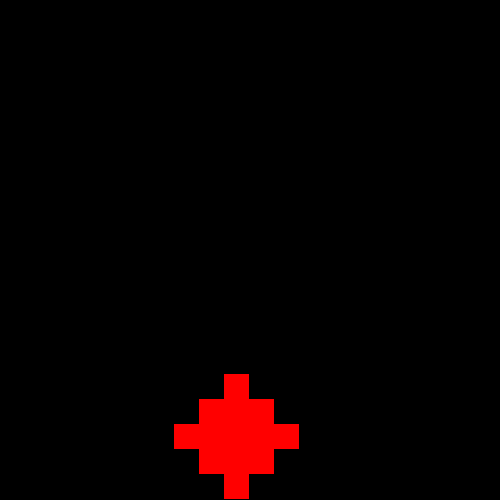
\includegraphics[scale = 0.4]{test_circle-2.png}
  
\includegraphics[scale = 0.4]{test_circle-23.png}
  \caption{Examples of circles}
\end{figure}

\begin{figure}[H]
  \centering
  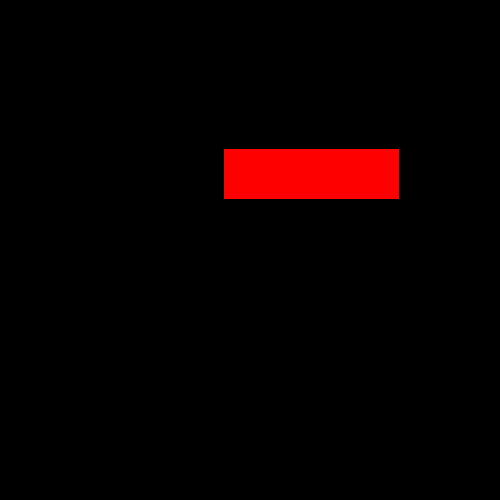
\includegraphics[scale = 0.4]{test_rect-39.png}
  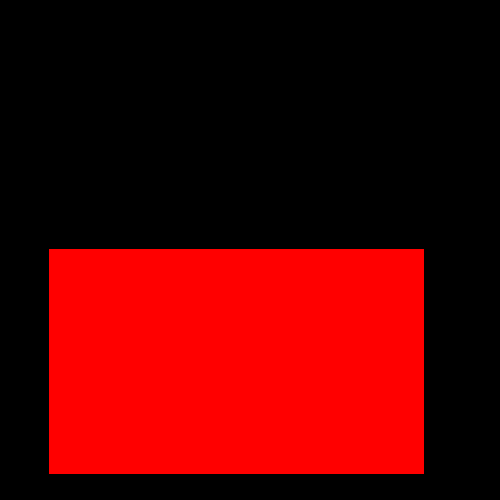
\includegraphics[scale = 0.4]{test_rect-13.png}
  \caption{Examples of rectangles}
\end{figure}
Each pixel represents an input, the images has a size of \textbf{20 x 20} pixels basically the perceptron
deals with \textbf{400} inputs then for each of these creates a weight, basically having
\textbf{400} weights, I know is too much, to train this kind of models is not easy because we
need to recollect massive datasets, for that reason I program this thing to have the capability to
generate its own dataset for its training, you can do that by manipulating the
\href{https://github.com/alecksandr26/machine-learning-code/blob/main/examples/perceptron_rectangle_circle/src/config.h}{config.h}.\\

The main idea of training and creating these kinds of models is to be used for problems where they
haven't been trained and be able to solve them, but obviously there is always going to be a
probability where the model gets a wrong answer, for that reason we always want to train this model
hardly with tons and tons of data.\\

You must  understand the larger our data set is, the less the probability of a wrong answer
from our model will be, and then after an hour of training the model, I tested with 1 hundred
random inputs where the neuron hadn't seen before and this was the result.
\begin{verbatim}
./main.out
 [INFO] Loading the brain
 [INFO] Brain detected
 [INFO] Brain loaded
 [INFO] Preparing the training data
 [INFO] Training data prepared
 [INFO] Training perceptron
 [INFO] Perceptron trained
 [INFO] Preparing the testing data
 [INFO] Testing data prepared
 [INFO] Testing perceptron
 [INFO] Perceptron tested
 [INFO] test fail data/test_rect-0.ppm
 [INFO] test fail data/test_rect-3.ppm
 [INFO] test fail data/test_circle-13.ppm
 [INFO] test fail data/test_rect-5.ppm
 [INFO] test fail data/test_circle-18.ppm
 [INFO] test fail data/test_rect-11.ppm
 [INFO] test fail data/test_rect-12.ppm
 [INFO] test fail data/test_circle-22.ppm
 [INFO] test fail data/test_circle-25.ppm
 [INFO] test fail data/test_circle-26.ppm
 [INFO] test fail data/test_rect-16.ppm
 [INFO] test fail data/test_rect-17.ppm
 [INFO] test fail data/test_rect-18.ppm
 [INFO] test fail data/test_rect-19.ppm
 [INFO] test fail data/test_rect-21.ppm
 [INFO] test fail data/test_circle-40.ppm
 [INFO] test fail data/test_rect-25.ppm
 [INFO] test fail data/test_rect-26.ppm
 [INFO] test fail data/test_rect-30.ppm
 [INFO] test fail data/test_circle-52.ppm
 [INFO] test fail data/test_circle-54.ppm
 [INFO] test fail data/test_rect-36.ppm
 [INFO] test fail data/test_rect-39.ppm
 [INFO] test fail data/test_rect-40.ppm
   76.0000000              76         100
 [INFO] Saving new brain
 [INFO] Brain saved
\end{verbatim}
And maybe the model needs more training or maybe it is because the problem is not linear separable,
we don't know, then I take all its \textbf{400} weights and put them in an image to have a graphical
representation of It's weights or It's brain.
\begin{figure}[H]
  \centering
  
\includegraphics{brain.png}
  \caption{The brain of the perceptron.}
\end{figure}

\subsubsection{The linearity of the problems:}
This is the main problem that makes the perceptron useless for general problems, this is
because the patters of most of the problems are not lineal, Obviously, it is hard to figure out when
a problem is linear and when it is not, because we can't imagine a hyperplane of several dimensions,
for reason it doesn't matter how much you train your model it wouldn't never converges for
general cases.\\
But when we mix several perceptrons making them to work together in a big structure of them
, we can deal with these non linear problemas, because making this structure forces each
perceptron to focus in an specific pattern of the big picture of the problem abstracting these patterns
giving us the posibility to classify non linear problems, you can imagine that now we are creating
several hiperplanes for each piece of the problem.\\
\begin{figure}[H]
  \centering
  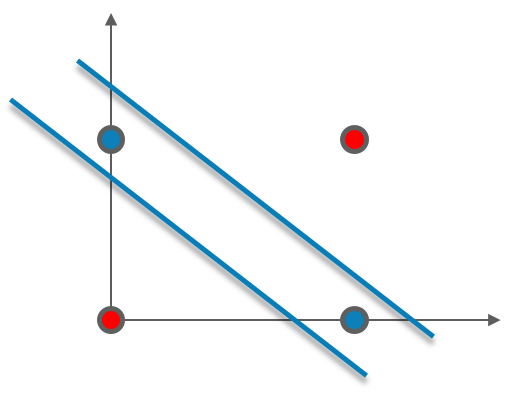
\includegraphics[scale = 0.5]{xor.png}
  \caption{A neural network dealing with an xor.}
\end{figure}
Well, here, as you can see, we need to have three neurons. One is in charge of learning the or
logic gate pattern and the second one is in charge of learning the nand logic gate, both of
them learn a patter of the big picture problem creating two hyperplane and abstracting the problem
to the third neuron which only needs the and logic gate.
\begin{figure}[H]
  \centering
  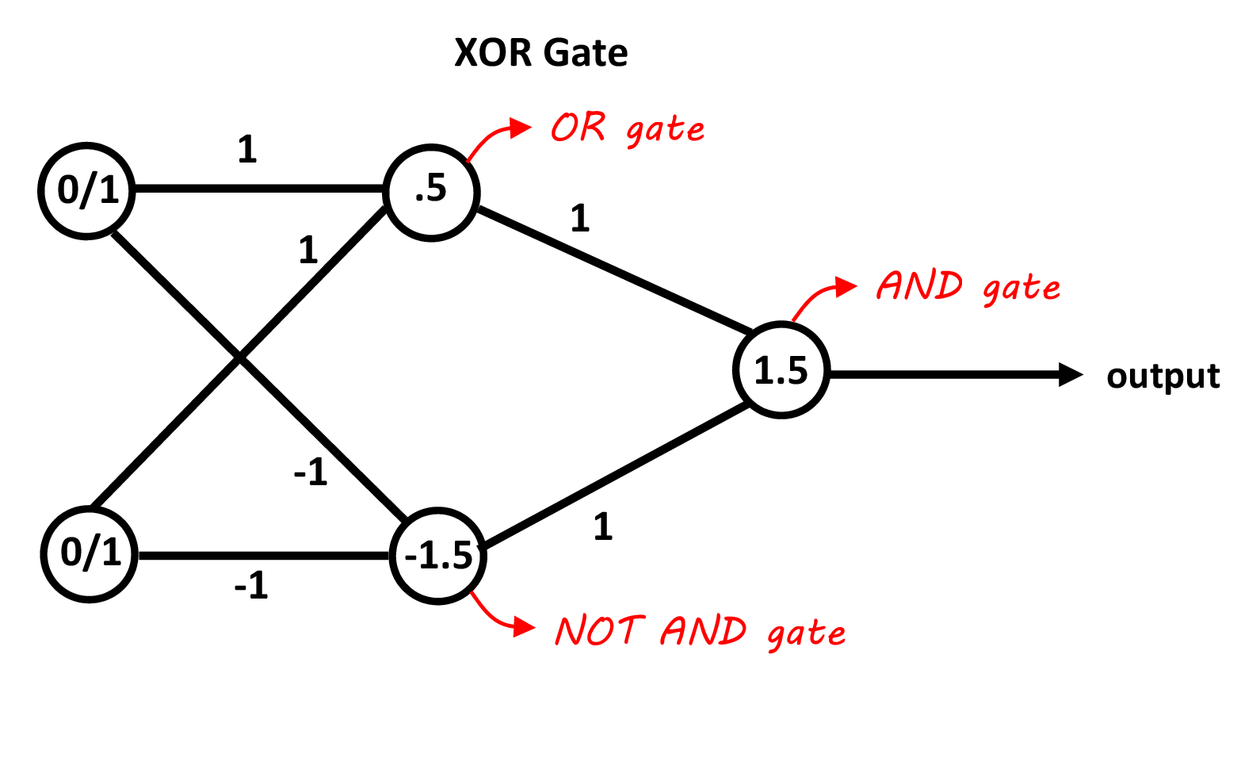
\includegraphics[scale = 0.5]{neurons.png}
  \caption{The structure of the nerual netowrk of the xor.}
\end{figure}
These structures are called neural networks and yeah, it is interesting when we create massive
structures of them.
\section{Conclusion:}
Perceptrons are limited to linearly separable problems, which means that they can only learn to
classify data that can be separated by a hyperplane. However, they have been used as building blocks
for more
complex neural network architectures that can handle more complex problems.\\
Overall, perceptrons are a simple and powerful tool for building basic binary classifiers, and
they have contributed significantly to the development of artificial intelligence and machine learning.

\section{References:}
\begin{itemize}
\item Zieba, J., PhD. (2022, December 16). How Do Neurons Work? The Scientist Magazine®.
  \url{https://www.the-scientist.com/university/brush-up-how-do-neurons-work-70839}
\item Action potentials and synapses. (2017, November 9). Queensland Brain Institute - University
  of Queensland.
  \url{https://qbi.uq.edu.au/brain-basics/brain/brain-physiology/action-potentials-and-synapses}
\item Perceptrons. (n.d.). \url{https://www.w3schools.com/ai/ai_perceptrons.asp}
\item Perceptron in Machine Learning - Javatpoint. (n.d.). www.javatpoint.com.
  \url{https://www.javatpoint.com/perceptron-in-machine-learning}
\item Training a Perceptron. (n.d.). \url{https://www.w3schools.com/ai/ai_training.asp}
\item Desmedt, S. (2019, May 12). The Math behind Neural Networks: Part 1 - The Rosenblatt Perceptron.
  CodeProject.
  \href{https://www.codeproject.com/Articles/4047091/The-Math-behind-Neural-Networks-Part-1-The-Rosenbl}{
    url}
\item Wikipedia contributors. (2023, March 21). Dot product. Wikipedia.
  \url{https://en.wikipedia.org/wiki/Dot_product}
\item Kilian Weinberger. (2018, July 9). Lecture 6 “Perceptron Convergence Proof” -Cornell
  CS4780 SP17 [Video]. YouTube. \url{https://www.youtube.com/watch?v=kObhWlqIeD8}
\item Kilian Weinberger. (2018, July 9). Lecture 5 “Perceptron” -Cornell
  CS4780 SP17 [Video]. YouTube. \url{https://www.youtube.com/watch?v=wl7gVvI-HuY}
\item Tsoding Daily. (2022, May 7).
  First Ancient Neural Network in C [Video]. \url{https://www.youtube.com/watch?v=WEk_grxrCcg}
\end{itemize}


\end{document}